\subsection{概述}
本节分为5部分, 分别介绍数据预处理, 以及对数据进行的五项数据处理, 并在部分章节中对数据进行了数据
可视化. 所有的代码都在src/data\_process.py中的类DataProcess中.
\begin{enumerate}
    \item 对HUMI, PRES, TEMP三列, 进行线性插值处理. 并对其中超过3倍标准差的高度异常
          数据, 修改为3倍标准差的数值.
    \item 假设PM指数最高为500, 对PM\_Dongsi, PM\_Dongsihuan, PM\_Nongzhanguan三列中
          超过500的数据, 修改为500PM指数进行异常值的处理.
    \item 修改cbwd列中值为"cv"的单元格, 其值用后项数据填充.
    \item 对DEWP和TEMP两列, 分别进行了0-1归一化和Z-Score归一化处理, 并将结果使用散点图的形式表示.
    \item 将北京的空气质量数据进行离散化, 按照空气质量分级标准, 计算出每个级别(或颜
          色值)对应的天数各有多少, 并将结果以饼图的形式进行可视化.
\end{enumerate}

\subsection{输入数据格式}
输入数据为csv表格形式存储的, 按日期排列的北京空气质量状况数据.
\begin{lstlisting}
    No,year,month,day,hour,season,PM_Dongsi,PM_Dongsihuan,PM_Nongzhanguan,PM_US Post,DEWP,HUMI,PRES,TEMP,cbwd,Iws,precipitation,Iprec
    1,2010,1,1,0,4,NA,NA,NA,NA,-21,43,1021,-11,NW,1.79,0,0
    2,2010,1,1,1,4,NA,NA,NA,NA,-21,47,1020,-12,NW,4.92,0,0
    3,2010,1,1,2,4,NA,NA,NA,NA,-21,43,1019,-11,NW,6.71,0,0
    4,2010,1,1,3,4,NA,NA,NA,NA,-21,55,1019,-14,NW,9.84,0,0
    5,2010,1,1,4,4,NA,NA,NA,NA,-20,51,1018,-12,NW,12.97,0,0
    6,2010,1,1,5,4,NA,NA,NA,NA,-19,47,1017,-10,NW,16.1,0,0
    7,2010,1,1,6,4,NA,NA,NA,NA,-19,44,1017,-9,NW,19.23,0,0
    8,2010,1,1,7,4,NA,NA,NA,NA,-19,44,1017,-9,NW,21.02,0,0
    9,2010,1,1,8,4,NA,NA,NA,NA,-19,44,1017,-9,NW,24.15,0,0
    
    ...
\end{lstlisting}

\subsection{数据预处理}
下面介绍数据集读入和预处理. 数据集读入和预处理在类DataProcessor中的函数
\_load\_data()中. 由于pandas的read\_csv()可以方便的对读入数据的日期进
行处理, 所以使用如下代码进行处理, 将数据的日期作为索引, 并让pandas自主推断日期格
式. 此外, 对数据中的NaN值进行了规定, 让Pandas可以正确读取NaN值, 而不是读成字符串.
\begin{lstlisting}
    self.raw_df = dataset
    # Read csv using pandas and store data in self.raw_dat and store data in
    # self.raw_data.
    dataset = pd.read_csv(
        in_file,
        parse_dates={"Date": ["year", "month", "day", "hour"]},
        date_parser=lambda x: datetime.strptime(x, "%Y %m %d %H"),
        infer_datetime_format=True,
        index_col="Date",
        na_values=["NaN", "?"],
    )
    self.raw_df = dataset
\end{lstlisting}

输入的数据格式如下:
\begin{lstlisting}
                        No  season  PM_Dongsi  PM_Dongsihuan  ...  cbwd    Iws  precipitation  Iprec
    Date                                                       ...                               
    2010-01-01 00:00:00   1       4        NaN            NaN  ...    NW   1.79            0.0    0.0
    2010-01-01 01:00:00   2       4        NaN            NaN  ...    NW   4.92            0.0    0.0
    2010-01-01 02:00:00   3       4        NaN            NaN  ...    NW   6.71            0.0    0.0
    2010-01-01 03:00:00   4       4        NaN            NaN  ...    NW   9.84            0.0    0.0
    2010-01-01 04:00:00   5       4        NaN            NaN  ...    NW  12.97            0.0    0.0
    2010-01-01 05:00:00   6       4        NaN            NaN  ...    NW  16.10            0.0    0.0
    2010-01-01 06:00:00   7       4        NaN            NaN  ...    NW  19.23            0.0    0.0
    2010-01-01 07:00:00   8       4        NaN            NaN  ...    NW  21.02            0.0    0.0
    2010-01-01 08:00:00   9       4        NaN            NaN  ...    NW  24.15            0.0    0.0
    2010-01-01 09:00:00  10       4        NaN            NaN  ...    NW  27.28            0.0    0.0
\end{lstlisting}

输入数据的统计信息如下:
\begin{lstlisting}
    --- Input data statistics:
<class 'pandas.core.frame.DataFrame'>
DatetimeIndex: 52584 entries, 2010-01-01 00:00:00 to 2015-12-31 23:00:00
Data columns (total 14 columns):
 #   Column           Non-Null Count  Dtype
---  ------           --------------  -----
 0   No               52584 non-null  int64
 1   season           52584 non-null  int64
 2   PM_Dongsi        25052 non-null  float64
 3   PM_Dongsihuan    20508 non-null  float64
 4   PM_Nongzhanguan  24931 non-null  float64
 5   PM_US Post       50387 non-null  float64
 6   DEWP             52579 non-null  float64
 7   HUMI             52245 non-null  float64
 8   PRES             52245 non-null  float64
 9   TEMP             52579 non-null  float64
 10  cbwd             52579 non-null  object
 11  Iws              52579 non-null  float64
 12  precipitation    52100 non-null  float64
 13  Iprec            52100 non-null  float64
dtypes: float64(11), int64(2), object(1)
\end{lstlisting}

\subsection{处理线性插值和高度异常数据}
本节介绍对HUMI, PRES和TEMP三列进行线性插值处理, 并截断其中超出三倍标准差的数据.\par

对线性插值和高度异常数据(超过3倍标准差)的数据的处理, 在类DataProcess中的函数
linear\_interpolate()中.\par

\subsubsection{实现介绍}
使用pandas的函数interpolate()对数据进行线性插值处理如下:
\begin{python}
    # Linear interpolate
    new_col = column.interpolate(
        method="linear", limit_direction="forward")
\end{python}

由于pandas是numpy的扩展, 所以很好的继承了numpy的特性, 例如下面用到的Boolean
Array.
对数据中超出三倍标准差的数据, 通过如下方式截断为三倍标准差:
\begin{python}
    # Process highly anomalous data that exceeds 3 standard deviations.
    std = column.std()
    mean = column.mean()
    new_col[column > mean + 3 * std] = 3 * std + mean
    new_col[column < mean - 3 * std] = 3 * std - mean
\end{python}

\subsubsection{处理结果}
使用样例数据进行测试. 测试结果中省略了不相关的列:
\begin{lstlisting}
    # Raw data before process.
                         No  season  ...  DEWP   HUMI  PRES  TEMP ...
    Date
    2010-01-01 00:00:00   1       4  ...   -21   43.0  1021   -11 ...
    2010-01-01 01:00:00   2       4  ...   -21   47.0  1020   -12 ...
    2010-01-01 02:00:00   3       4  ...   -21   43.0  1019   -11 ...
    2010-01-01 03:00:00   4       4  ...   -21   55.0  1019   -14 ...
    2010-01-01 04:00:00   5       4  ...   -20    NaN  1018   -12 ...
    2010-01-01 05:00:00   6       4  ...   -19   47.0  1017   -10 ...
    2010-01-01 06:00:00   7       4  ...   -19   44.0  1017    -9 ...
    2010-01-01 07:00:00   8       4  ...   -19  440.0  1017    -9 ...
    2010-01-01 08:00:00   9       4  ...   -19   44.0  1017    -9 ...
    2010-01-01 09:00:00  10       4  ...   -20   37.0  1017    -8 ...

    # Run log.
    Linear interpolate and process highly anomalous data in HUMI.
    Modified 1 cells.
    Linear interpolate and process highly anomalous data in PRES.
    Modified 0 cells.
    Linear interpolate and process highly anomalous data in PRES.
    Modified 0 cells.

    # Processed data.
                         No  season  ...  DEWP   HUMI  PRES  TEMP ...
    Date
    2010-01-01 00:00:00   1       4  ...   -21   43.0  1021   -11 ...
    2010-01-01 01:00:00   2       4  ...   -21   47.0  1020   -12 ...
    2010-01-01 02:00:00   3       4  ...   -21   43.0  1019   -11 ...
    2010-01-01 03:00:00   4       4  ...   -21   55.0  1019   -14 ...
    2010-01-01 04:00:00   5       4  ...   -20   51.0  1018   -12 ...
    2010-01-01 05:00:00   6       4  ...   -19   47.0  1017   -10 ...
    2010-01-01 06:00:00   7       4  ...   -19   44.0  1017    -9 ...
    2010-01-01 07:00:00   8       4  ...   -19  440.0  1017    -9 ...
    2010-01-01 08:00:00   9       4  ...   -19   44.0  1017    -9 ...
    2010-01-01 09:00:00  10       4  ...   -20   37.0  1017    -8 ...
\end{lstlisting}
可以看到HUMI中的NaN被插值为51.0.

对完整数据集进行测试, 根据输出日志可以看到, 三列中均有数据被进行过插值或修改到三倍标准差内.
\begin{lstlisting}
Linear interpolate and process highly anomalous data in HUMI.
Modified 339 cells.
Linear interpolate and process highly anomalous data in PRES.
Modified 339 cells.
Linear interpolate and process highly anomalous data in PRES.
Modified 5 cells.
\end{lstlisting}

\subsection{处理PM指数异常值}
本节介绍对PM\_Dongsi, PM\_Dongsihuan和PM\_Nongzhanguan三列中PM指数超过500的异常
数据进行处理. 处理方法为将其截断为500.\par

\subsection{实现介绍}
类似上一节中提到的方式, 使用pandas中DataFrame的Boolean Array对每一列col中的异常数据进行处理:
\begin{lstlisting}
    def process(col):
        cp = col.copy()
        print(f"Handled {len([x for x in cp[cp > 500]])} values")
        cp[cp > 500] = 500

        return cp
\end{lstlisting}

\subsection{处理结果}
对样例数据进行测试, 测试结果中省略了不相关的列:
\begin{lstlisting}
    # Raw data before process.
                         No  season  PM_Dongsi  PM_Dongsihuan  PM_Nongzhanguan  ...
    Date
    2010-01-01 00:00:00   1       4        NaN            NaN              NaN  ...
    2010-01-01 01:00:00   2       4        NaN            NaN              NaN  ...
    2010-01-01 02:00:00   3       4        NaN            NaN              NaN  ...
    2010-01-01 03:00:00   4       4        NaN            NaN            858.0  ...
    2010-01-01 04:00:00   5       4        NaN           39.0              NaN  ...
    2010-01-01 05:00:00   6       4        NaN            NaN              NaN  ...
    2010-01-01 06:00:00   7       4        NaN         1871.0              NaN  ...
    2010-01-01 07:00:00   8       4       17.0            NaN              NaN  ...
    2010-01-01 08:00:00   9       4        NaN            NaN              NaN  ...
    2010-01-01 09:00:00  10       4        NaN            NaN              NaN  ...
    
    # Run log.
    Handle values larger than 500 in PM_Dongsi.
    Handled 0 values
    Handle values larger than 500 in PM_Dongsihuan.
    Handled 1 values
    Handle values larger than 500 in PM_Nongzhanguan.
    Handled 1 values
    
    # Processed data.
                         No  season  PM_Dongsi  PM_Dongsihuan  PM_Nongzhanguan  ...
    Date
    2010-01-01 00:00:00   1       4        NaN            NaN              NaN  ...
    2010-01-01 01:00:00   2       4        NaN            NaN              NaN  ...
    2010-01-01 02:00:00   3       4        NaN            NaN              NaN  ...
    2010-01-01 03:00:00   4       4        NaN            NaN            500.0  ...
    2010-01-01 04:00:00   5       4        NaN           39.0              NaN  ...
    2010-01-01 05:00:00   6       4        NaN            NaN              NaN  ...
    2010-01-01 06:00:00   7       4        NaN          500.0              NaN  ...
    2010-01-01 07:00:00   8       4       17.0            NaN              NaN  ...
    2010-01-01 08:00:00   9       4        NaN            NaN              NaN  ...
    2010-01-01 09:00:00  10       4        NaN            NaN              NaN  ...
\end{lstlisting}
可以看到, PM\_Dongsihuan列中值为1871.0的数值被截断为500.0; PM\_Nongzhanguan中值
为858.0的被截断为500.0. 对不超过500.0的值不进行处理.\par

对完整数据集进行测试, 根据输出日志可以看到, 三列中均有PM指数超过500的异常数据被
进行了截断.
\begin{lstlisting}
Handle values larger than 500 in PM_Dongsi.
Handled 70 values
Handle values larger than 500 in PM_Dongsihuan.
Handled 75 values
Handle values larger than 500 in PM_Nongzhanguan.
Handled 81 values
\end{lstlisting}

\subsection{处理cbwd中值为"cv"的单元格}
% TODO: Finished this part.
本节介绍对cbwd中值为"cv"的单元格使用后项数据填充.

\subsection{实现介绍}
关键代码段如下:
\begin{lstlisting}[language=Python]
    for i in range(len(cbwd.index), 1, -1):
        if cbwd[i-1] == 'cv':
            cnt += 1
        cbwd[i-1] = cbwd[i] if cbwd[i-1] == "cv" else cbwd[i-1]
\end{lstlisting}
由于是从后往前替换, 所以即便是多个相连的cv, 也能完成替换.

\subsection{处理结果}
使用样例数据进行测试, 测试结果中省略了不相关的列:
\begin{lstlisting}
                         No  season  ... cbwd    Iws  precipitation  Iprec
    Date
    2010-01-01 00:00:00   1       4  ...   NW   1.79              0      0
    2010-01-01 01:00:00   2       4  ...   NW   4.92              0      0
    2010-01-01 02:00:00   3       4  ...   NW   6.71              0      0
    2010-01-01 03:00:00   4       4  ...   NW   9.84              0      0
    2010-01-01 04:00:00   5       4  ...   NW  12.97              0      0
    2010-01-01 05:00:00   6       4  ...   NW  16.10              0      0
    2010-01-01 06:00:00   7       4  ...   NW  19.23              0      0
    2010-01-01 07:00:00   8       4  ...   cv  21.02              0      0
    2010-01-01 08:00:00   9       4  ...   NW  24.15              0      0
    2010-01-01 09:00:00  10       4  ...   NW  27.28              0      0
    
    ...
    Modified 1 cells whose value is 'cv' in column 'cbwd'.
                         No  season  ... cbwd    Iws  precipitation  Iprec
    Date
    2010-01-01 00:00:00   1       4  ...   NW   1.79              0      0
    2010-01-01 01:00:00   2       4  ...   NW   4.92              0      0
    2010-01-01 02:00:00   3       4  ...   NW   6.71              0      0
    2010-01-01 03:00:00   4       4  ...   NW   9.84              0      0
    2010-01-01 04:00:00   5       4  ...   NW  12.97              0      0
    2010-01-01 05:00:00   6       4  ...   NW  16.10              0      0
    2010-01-01 06:00:00   7       4  ...   NW  19.23              0      0
    2010-01-01 07:00:00   8       4  ...   NW  21.02              0      0
    2010-01-01 08:00:00   9       4  ...   NW  24.15              0      0
    2010-01-01 09:00:00  10       4  ...   NW  27.28              0      0
\end{lstlisting}
可以看到原本是cv的一行被替换为了下一行中的NW.

\subsection{归一化处理和散点图表示}
本节对DEWP和TEMP两列分别使用Pandas进行了0-1归一化和Z-Score归一化处理,
并将结果使用matplotlib绘制饼图进行可视化处理.

\subsubsection{实现介绍}
0-1正规化, 将原始数据缩放到[0, 1]区间内:
\begin{equation}
    \frac{x-\min}{\max - \min}
\end{equation}
但是缺点是当新数据加入的时候, 可能导致最大和最小值发生变化, 从而需要重新计算.

z-Score, 将原始数据转换为标准正态分布:
\begin{equation}
    \frac{x-\mu}{\sigma}
\end{equation}
但是缺点是对原始数据的分布有要求, 即原始数据的分布必须是近似正态分布的.

\begin{python}
    min = df["DEWP"].min()
    max = df["DEWP"].max()

    # 0-1 normalization.
    def norm01(x, min, max): return (x - min) / (max - min)
    def norm01_col(col): return [norm01(col[i], min, max) for i in
                                 range(len(col))]

    df["DEWP"] = norm01_col(df["DEWP"])
    print(f"0-1 nomalized column 'DEWP'.")

    # Normalize column TEMP with Z-Score
    def norm_z(x, mean, std): return (x - mean) / std
    mean = df["TEMP"].mean()
    std = df["TEMP"].std()
    def norm_z_col(col): return [norm_z(col[i], mean, std) for i in
                                 range(len(col))]
    df["TEMP"] = norm_z_col(df["TEMP"])
    print(f"z-score normalized column 'TEMP'.") 
\end{python}

\subsubsection{处理结果}
\begin{lstlisting}
                         No  season  ...  DEWP   HUMI  PRES  TEMP ...
    Date
    2010-01-01 00:00:00   1       4  ...   -21   43.0  1021   -11 ...
    2010-01-01 01:00:00   2       4  ...   -21   47.0  1020   -12 ...
    2010-01-01 02:00:00   3       4  ...   -21   43.0  1019   -11 ...
    2010-01-01 03:00:00   4       4  ...   -21   55.0  1019   -14 ...
    2010-01-01 04:00:00   5       4  ...   -20    NaN  1018   -12 ...
    2010-01-01 05:00:00   6       4  ...   -19   47.0  1017   -10 ...
    2011-01-01 06:00:00   7       4  ...   -19   44.0  1017    -9 ...
    2010-01-01 07:00:00   8       4  ...   -19  440.0  1017    -9 ...
    2010-01-01 08:00:00   9       4  ...   -19   44.0  1017    -9 ...
    2010-01-01 09:00:00  10       4  ...   -20   37.0  1017    -8 ...

    ...
    0-1 nomalized column 'DEWP'.
    z-score normalized column 'TEMP'.
                         No  season  ...  DEWP   HUMI  PRES      TEMP ...
    Date
    2010-01-01 00:00:00   1       4  ...   0.0   43.0  1021 -0.271607 ...
    2010-01-01 01:00:00   2       4  ...   0.0   47.0  1020 -0.814822 ...
    2010-01-01 02:00:00   3       4  ...   0.0   43.0  1019 -0.271607 ...
    2010-01-01 03:00:00   4       4  ...   0.0   55.0  1019 -1.901251 ...
    2010-01-01 04:00:00   5       4  ...   0.5   51.0  1018 -0.814822 ...
    2010-01-01 05:00:00   6       4  ...   1.0   47.0  1017  0.271607 ...
    2010-01-01 06:00:00   7       4  ...   1.0   44.0  1017  0.814822 ...
    2010-01-01 07:00:00   8       4  ...   1.0  440.0  1017  0.814822 ...
    2010-01-01 08:00:00   9       4  ...   1.0   44.0  1017  0.814822 ...
    2010-01-01 09:00:00  10       4  ...   0.5   37.0  1017  1.358036 ...
\end{lstlisting}
可以看到DEWP中数据被0-1正规化, 而TEMP中数据被z-score正规化.

\subsubsection{可视化结果}
由于测试集的数据规模较小, 不能很好的体现正规化后的特征,
因此使用北京PM完整数据集对0-1正规化和z-score正规化的数据使用散点图进行展示如图.
\begin{figure}
    \centering
    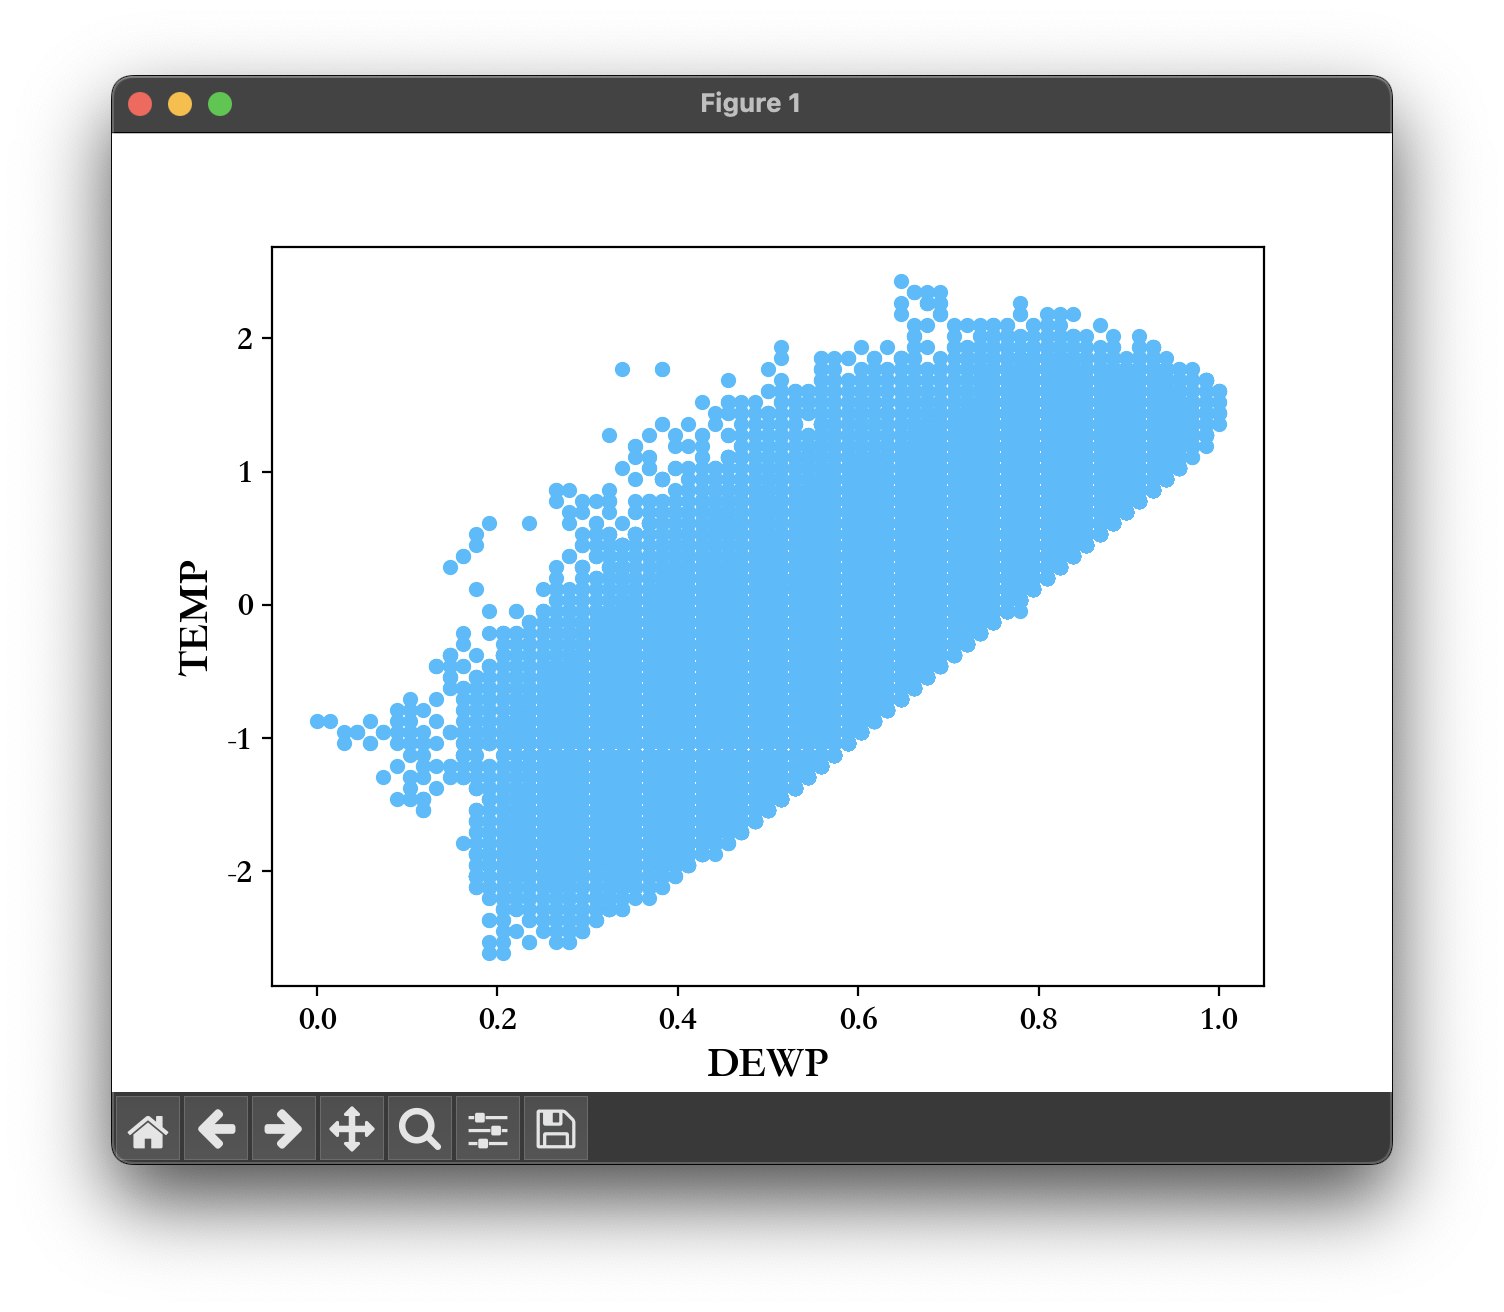
\includegraphics[width=0.8\textwidth]{figures/normalized-scatter.png}
    \label{fig:0-1正规化和z-score正规化散点图}
    \caption{0-1正规化和z-score正规化散点图}
\end{figure}

\subsection{空气质量数据离散化和饼图表示}
本节介绍将北京的空气质量数据进行离散化, 按照空气质量分级表存, 计算出每个级别对应
的挺熟, 并将结果以饼图的形式进行可视化. 对每一个PM来源均分别进行饼图可视化, 以便于比较.

\subsubsection{空气质量分级标准}
参考如表~\ref{tab:空气质量分级标准}空气质量分级标准:
\begin{table}[ht!]
    \centering
    \begin{tabular}{|l|l|}
        \hline
        空气质量指数(AQI) & 空气质量指数级别(状况)              \\
        \hline
        \hline
        0-50        & Excellent(优)              \\
        51-100      & Good(良)                   \\
        101-150     & Lightly Polluted(轻度污染)    \\
        151-200     & Moderately Polluted(中度污染) \\
        201-300     & Heavily Polluted(重度污染)    \\
        300+        & Severely Polluted(严重污染)   \\
        \hline
    \end{tabular}
    \caption{空气质量分级标准}
    \label{tab:空气质量分级标准}
\end{table}

\subsubsection{实现介绍}
由于不同观测数据来源的PM数据有差异, 故使用如下函数对各站点PM数据分别进行离散化.
\begin{python}
    # Discretize PM_Dongsi into PM_Dongsi_AQI:
    def discretize_pm(column, discretized_column):
        for row in column:
            if 0 <= row <= 50:
                discretized_column.append(aqis.excellent._value_)
            elif 51 <= row <= 100:
                discretized_column.append(aqis.good._value_)
            elif 101 <= row <= 150:
                discretized_column.append(aqis.lightly_polluted._value_)
            elif 151 <= row <= 200:
                discretized_column.append(aqis.moderately_polluted._value_)
            elif 201 <= row <= 300:
                discretized_column.append(aqis.heavily_polluted._value_)
            elif row > 300:
                discretized_column.append(aqis.severely_polluted._value_)
            else:
                # Handle NaN value.
                discretized_column.append(row)
\end{python}

数据可视化部分, 首先统计了各空气质量等级的天数:
\begin{python}
    classes = [self.aqicategories.excellent._value_,
    self.aqicategories.good._value_,
    self.aqicategories.lightly_polluted._value_,
    self.aqicategories.moderately_polluted._value_,
    self.aqicategories.heavily_polluted._value_,
    self.aqicategories.severely_polluted._value_]

    def count(col):
    '''
    Count AQI categories. Ignore NaN values.
    '''
    rslt = [0 for i in range(len(classes))]
    for row in col:
     if row in classes:
         rslt[classes.index(row)] += 1
    return rslt
\end{python}

然后对数据绘制饼图进行可视化:
\begin{python}
    data_dongsi = count(df["PM_Dongsi_AQI"])
    data_dongsihuan = count(df["PM_Dongsihuan_AQI"])
    data_nongzhanguan = count(df["PM_Nongzhanguan_AQI"])
    data_us = count(df["PM_US Post_AQI"])

    def draw_sub_pie(data, ax_x, ax_y):
    '''
    Draw subplot of pie.
    '''
    def get_absolute(pct, allvals):
        '''
        Get absolute value of days from percentage.
        '''
        absolute = int(np.round(pct/100.*np.sum(allvals)))
        return "{:.1f}%\n({:d} days)".format(pct, absolute)

    wedges, texts, autotexts = ax.pie(data, wedgeprops=dict(
        width=0.618), startangle=90, autopct=lambda pct: get_absolute(pct, data))
    bbox_props = dict(boxstyle="square,pad=0.3",
                      fc="w", ec="k", lw=0.72)
    kw = dict(arrowprops=dict(arrowstyle="-"),
              bbox=bbox_props, zorder=0, va="center")

    # Compute angle of label line
    for i, p in enumerate(wedges):
        ang = (p.theta2 - p.theta1)/2. + p.theta1
        y = np.sin(np.deg2rad(ang))
        x = np.cos(np.deg2rad(ang))
        horizontalalignment = {-1: "right", 1: "left"}[int(np.sign(x))]
        connectionstyle = "angle,angleA=0,angleB={}".format(ang)
        kw["arrowprops"].update({"connectionstyle": connectionstyle})
        ax.annotate(classes[i] + " " + zh_classes[i], xy=(x, y), xytext=(
            1.35*np.sign(x), 1.2*y), horizontalalignment=horizontalalignment, **kw)

    
    # Draw PM_Dongsi pie plot.
    fig, ax = plt.subplots(figsize=(
        12, 8), subplot_kw=dict(aspect="equal"))
    draw_sub_pie(data_dongsi, 0, 0)
    ax.set_title("Dongsi PM AQI")
    plt.show()
    
    ...
\end{python}

\subsubsection{处理结果}
在样例数据上进行处理得到的结果如下, 由于新增四列后表格太宽, 所以进行了换行:
\begin{lstlisting}
    ...  PM_Dongsi  PM_Dongsihuan  PM_Nongzhanguan  PM_US Post  ...    
    ...                                                         ...
    ...        NaN            NaN              NaN         NaN  ...    
    ...        NaN            NaN              NaN         NaN  ...    
    ...        NaN            NaN              NaN         NaN  ...    
    ...        NaN            NaN            500.0         NaN  ...    
    ...        NaN           39.0              NaN         NaN  ...    
    ...        NaN            NaN              NaN      1818.0  ...    
    ...        NaN          500.0              NaN       383.0  ...    
    ...       17.0            NaN              NaN        12.0  ...    
    ...        NaN            NaN              NaN         NaN  ...    
    ...        NaN            NaN              NaN         NaN  ...    

     PM_Dongsi_AQI  PM_Dongsihuan_AQI PM_Nongzhanguan_AQI     PM_US Post_AQI
                                                                            
               NaN                NaN                 NaN                NaN
               NaN                NaN                 NaN                NaN
               NaN                NaN                 NaN                NaN
               NaN                NaN   Severely Polluted                NaN
               NaN          Excellent                 NaN                NaN
               NaN                NaN                 NaN  Severely Polluted
               NaN  Severely Polluted                 NaN  Severely Polluted
         Excellent                NaN                 NaN          Excellent
               NaN                NaN                 NaN                NaN
               NaN                NaN                 NaN                NaN
\end{lstlisting}
可以看到对非NaN的值, 都进行了正确的对应离散化.

在完整的Bejing PM数据集上处理的各观测数据的统计信息如下:
\begin{lstlisting}
PM_Dongsi statistics:
    Excellent[10576]
    Good[6268]
    Lightly Polluted[3578]
    Moderately Polluted[1942]
    Heavily Polluted[1910]
    Severely Polluted[778]

PM_Dongsihuan statistics:
    Excellent[8104]
    Good[5408]
    Lightly Polluted[3143]
    Moderately Polluted[1683]
    Heavily Polluted[1416]
    Severely Polluted[754]

PM_Nongzhanguan statistics:
    Excellent[10730]
    Good[6259]
    Lightly Polluted[3408]
    Moderately Polluted[1934]
    Heavily Polluted[1697]
    Severely Polluted[903]

PM_US Post statistics:
    Excellent[20050]
    Good[12576]
    Lightly Polluted[7414]
    Moderately Polluted[4274]
    Heavily Polluted[4016]
    Severely Polluted[2057]
\end{lstlisting}

\subsubsection{可视化结果}
PM\_Dongsi的可视化结果如图~\ref{fig:PMDongsi的AQI离散化}.

\begin{figure}[ht!]
    \centering
    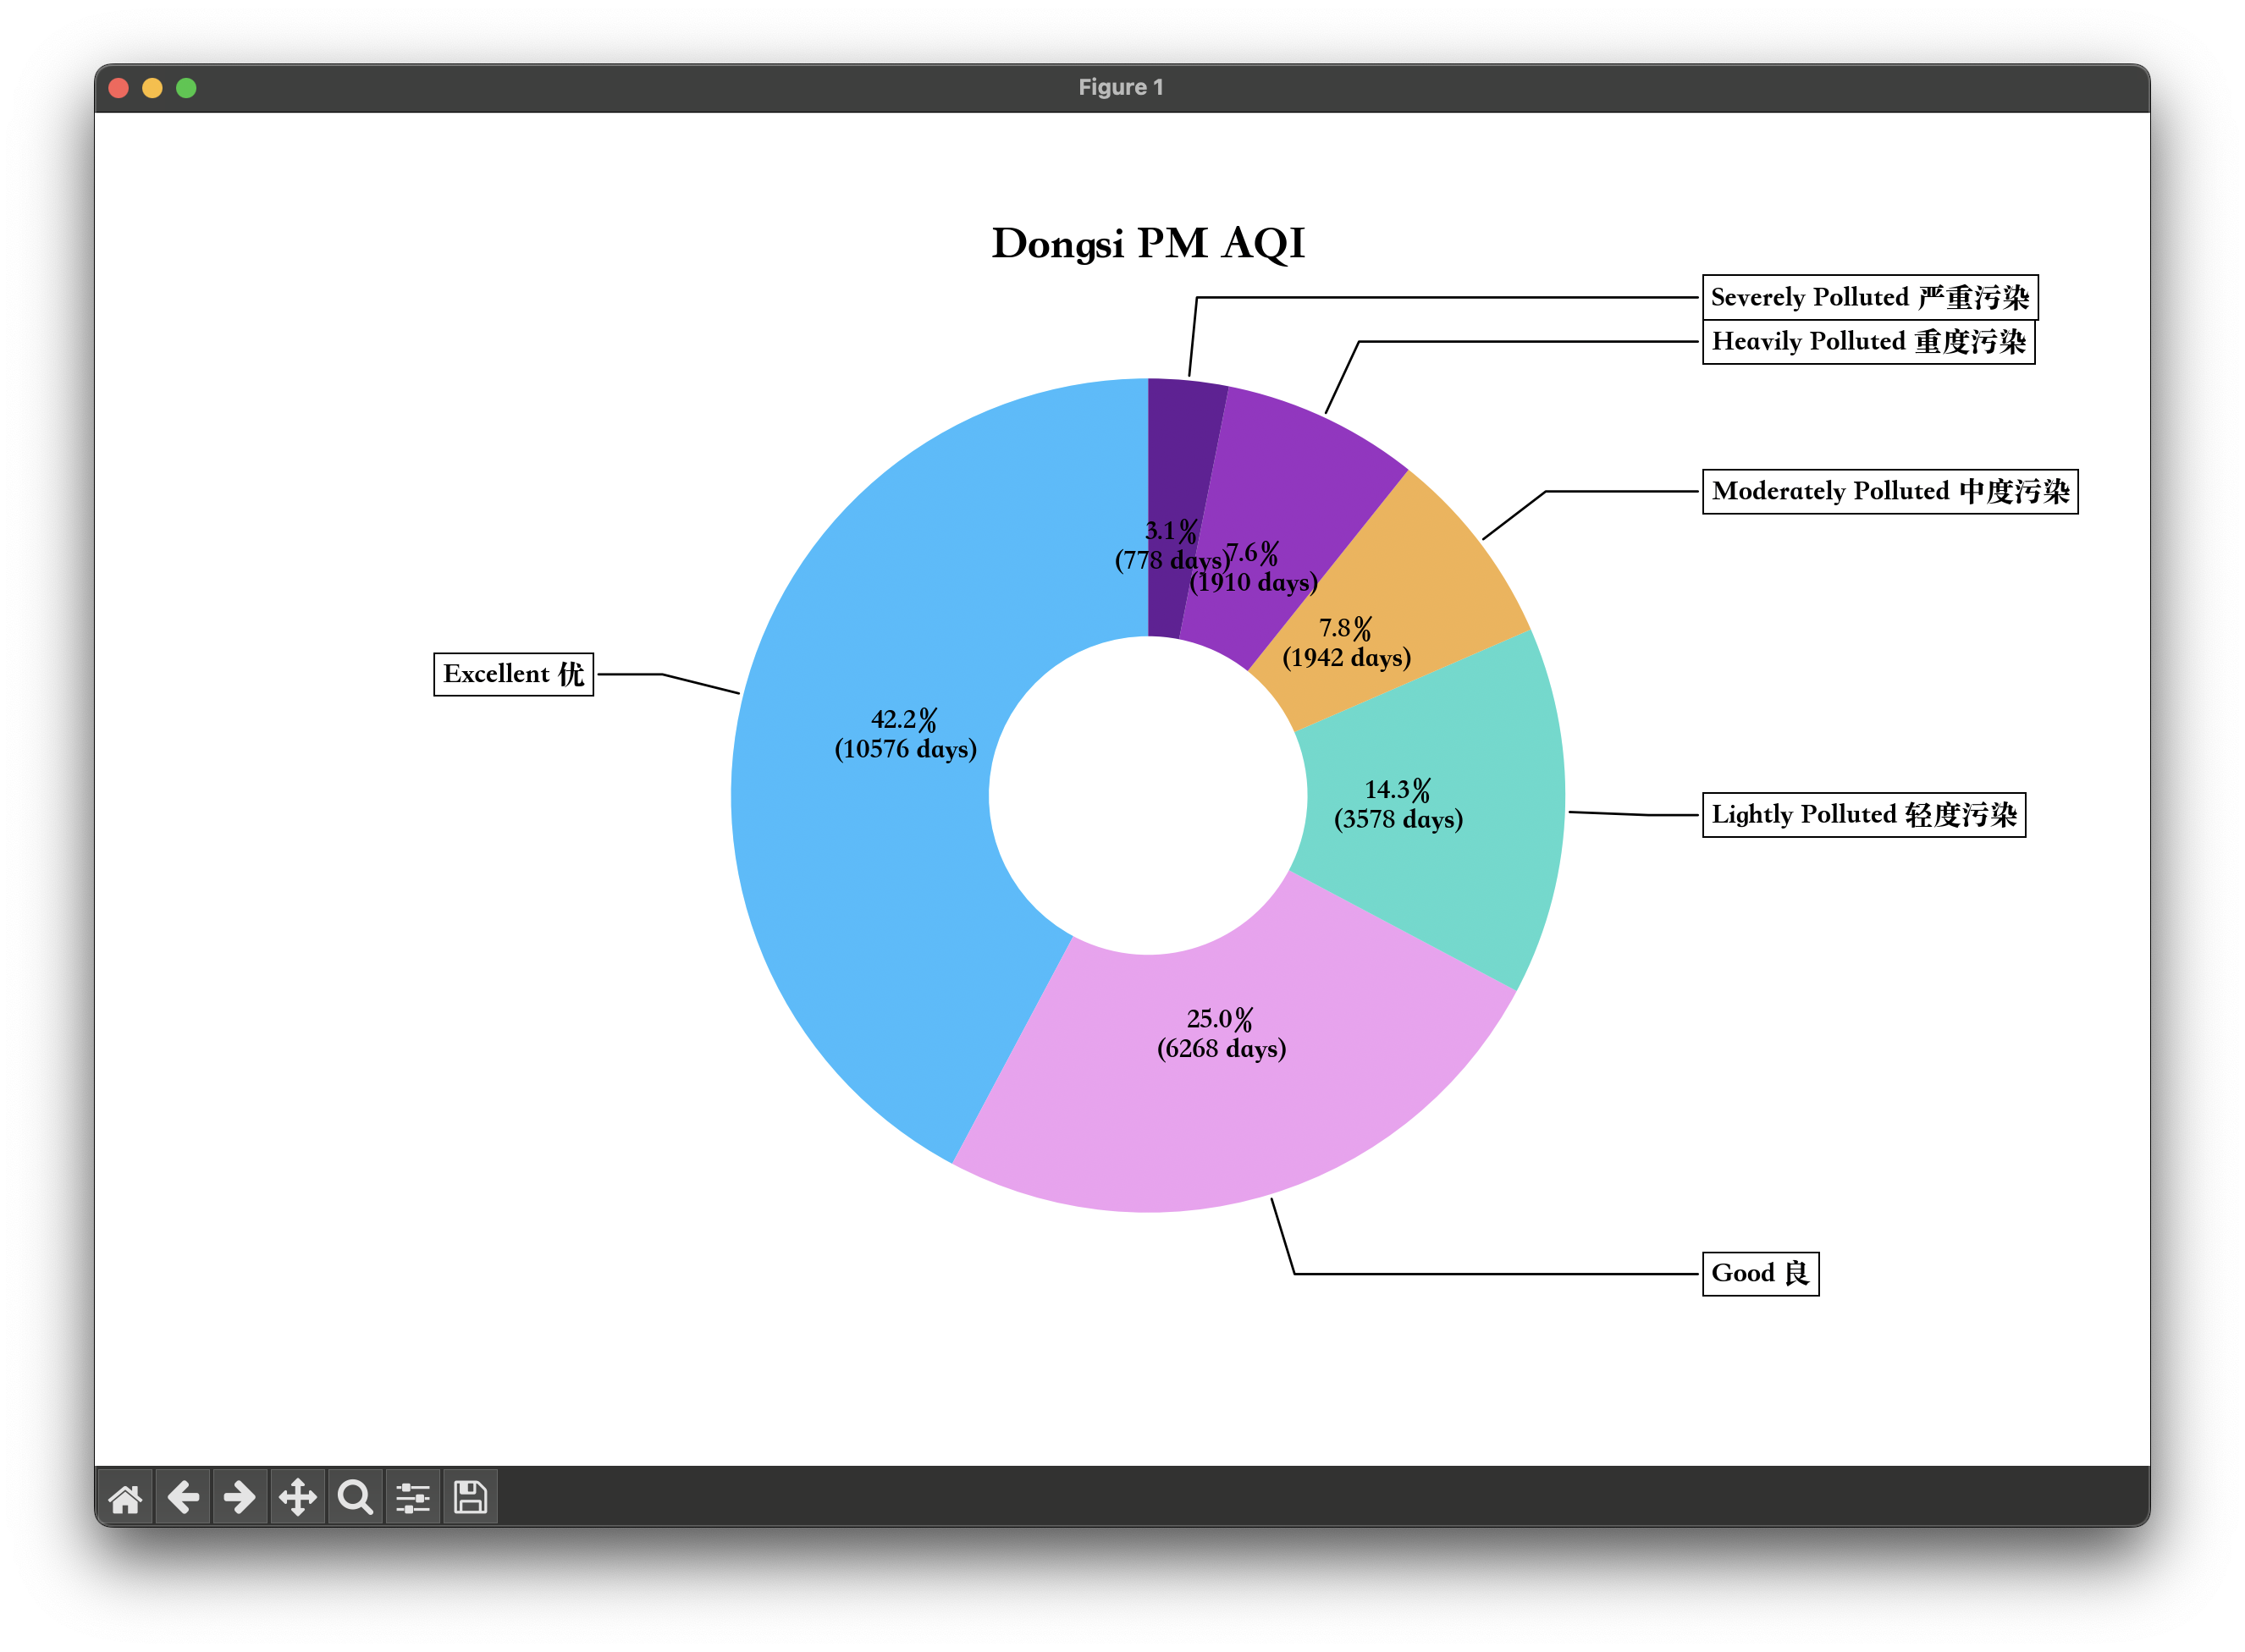
\includegraphics[width=0.8\textwidth]{discretize-aqi-dongsi.png}
    \caption{PM\_Dongsi的AQI离散化}
    \label{fig:PMDongsi的AQI离散化}
\end{figure}

PM\_Dongsihuan的可视化结果如图~\ref{fig:PMDongsihuan的AQI离散化}

\begin{figure}[ht!]
    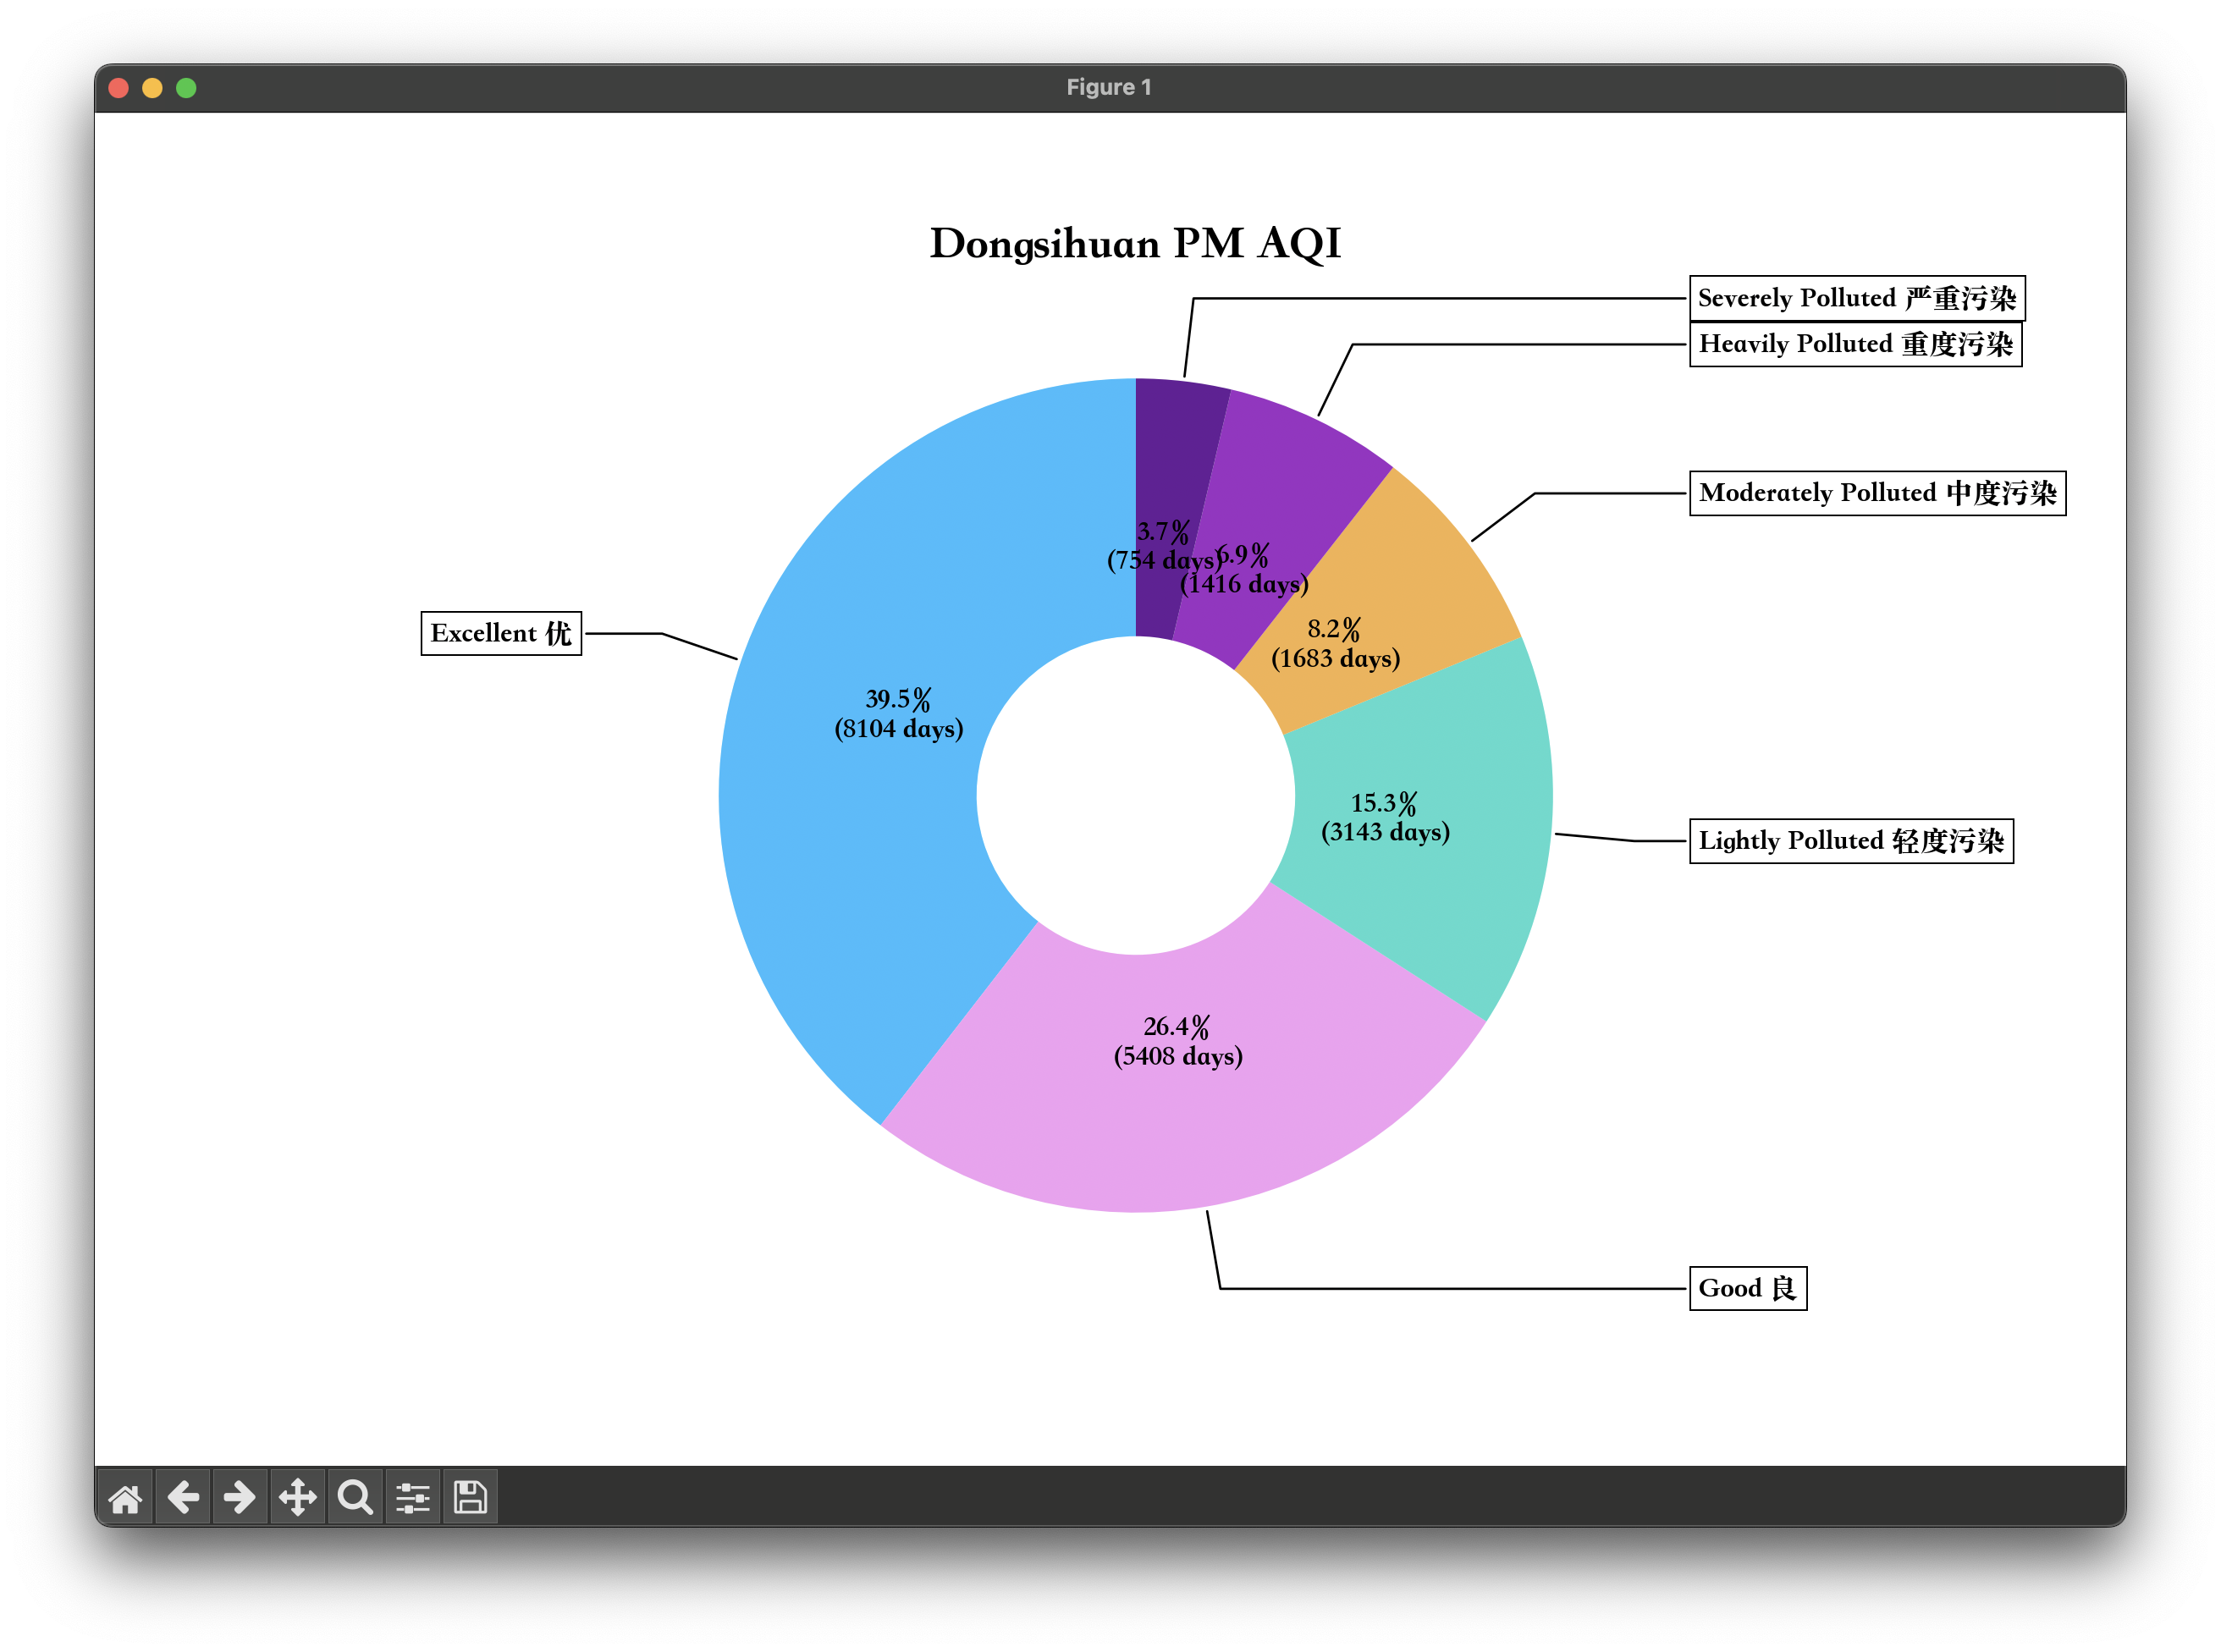
\includegraphics[width=0.8\textwidth]{discretize-aqi-dongsihuan.png}
    \centering
    \caption{PM\_Dongsihuan的AQI离散化}
    \label{fig:PMDongsihuan的AQI离散化}
\end{figure}

PM\_Nongzhanguan的可视化结果如图~\ref{fig:PMNongzhanguan的AQI离散化}
\begin{figure}[ht!]
    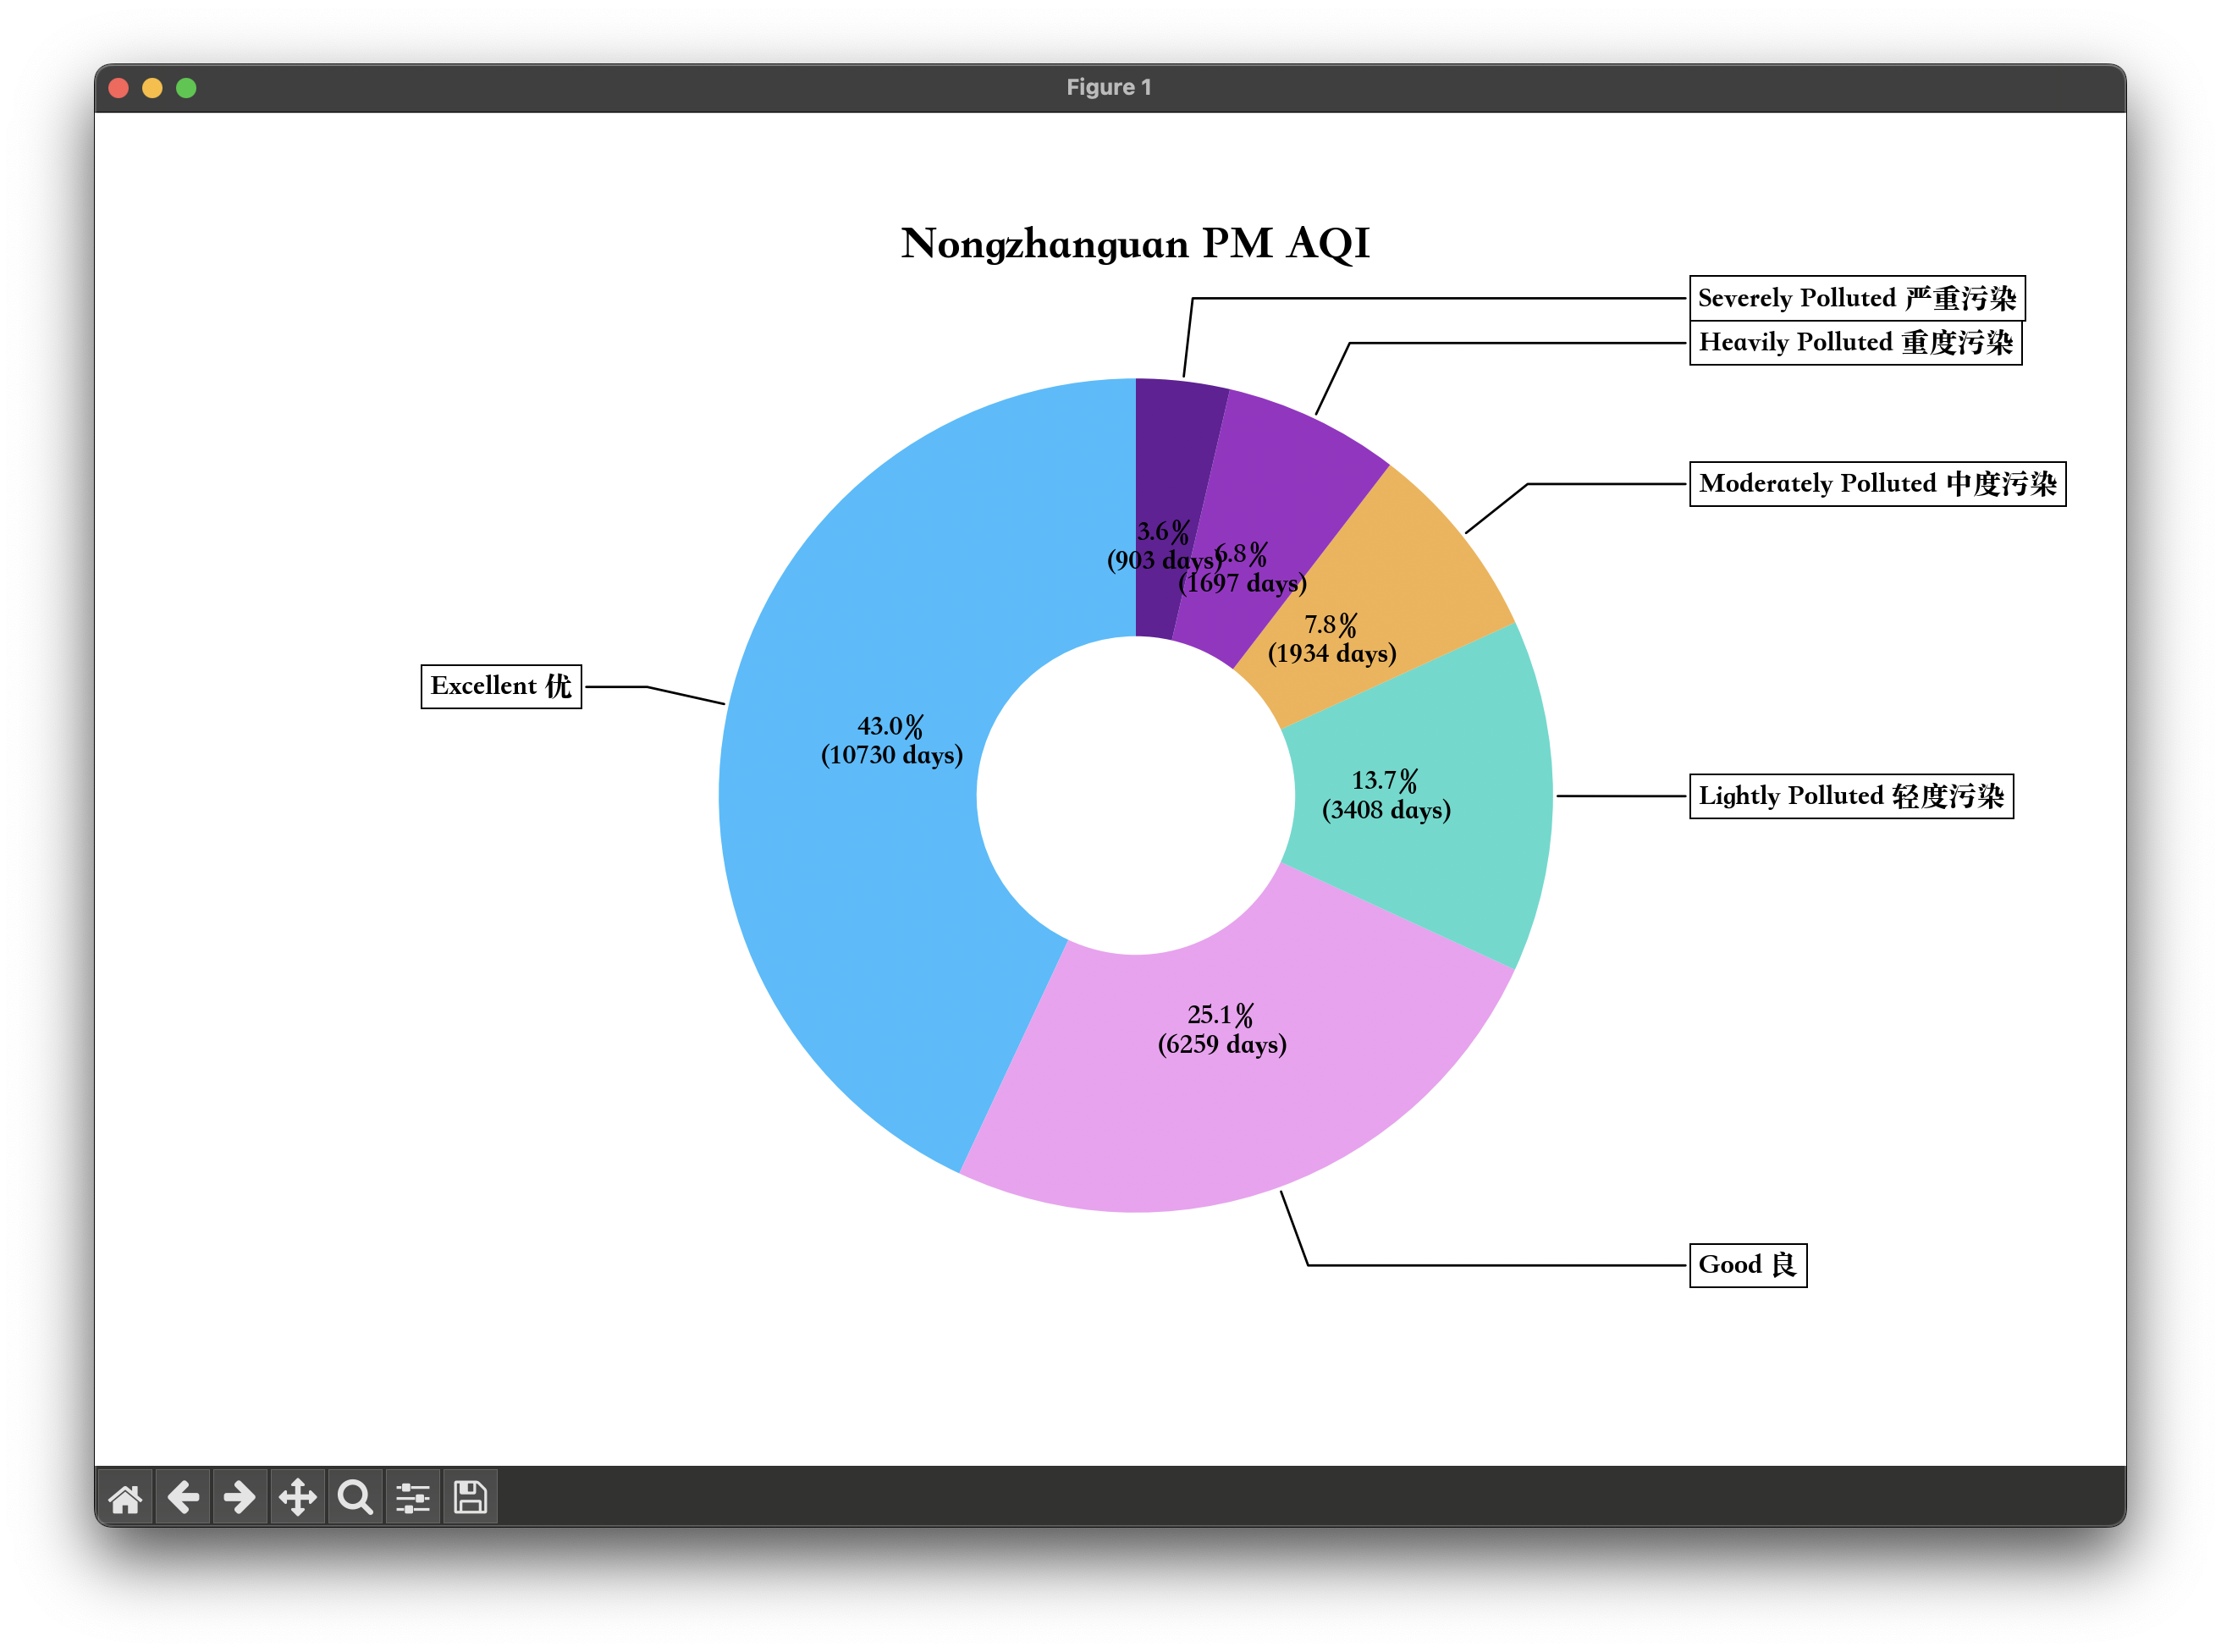
\includegraphics[width=0.8\textwidth]{discretize-aqi-nongzhanguan.png}
    \centering
    \caption{PM\_Nongzhanguan的AQI离散化}
    \label{fig:PMNongzhanguan的AQI离散化}
\end{figure}

PM\_US Post的可视化结果如图~\ref{fig:PMUS Post的AQI离散化}
\begin{figure}[ht!]
    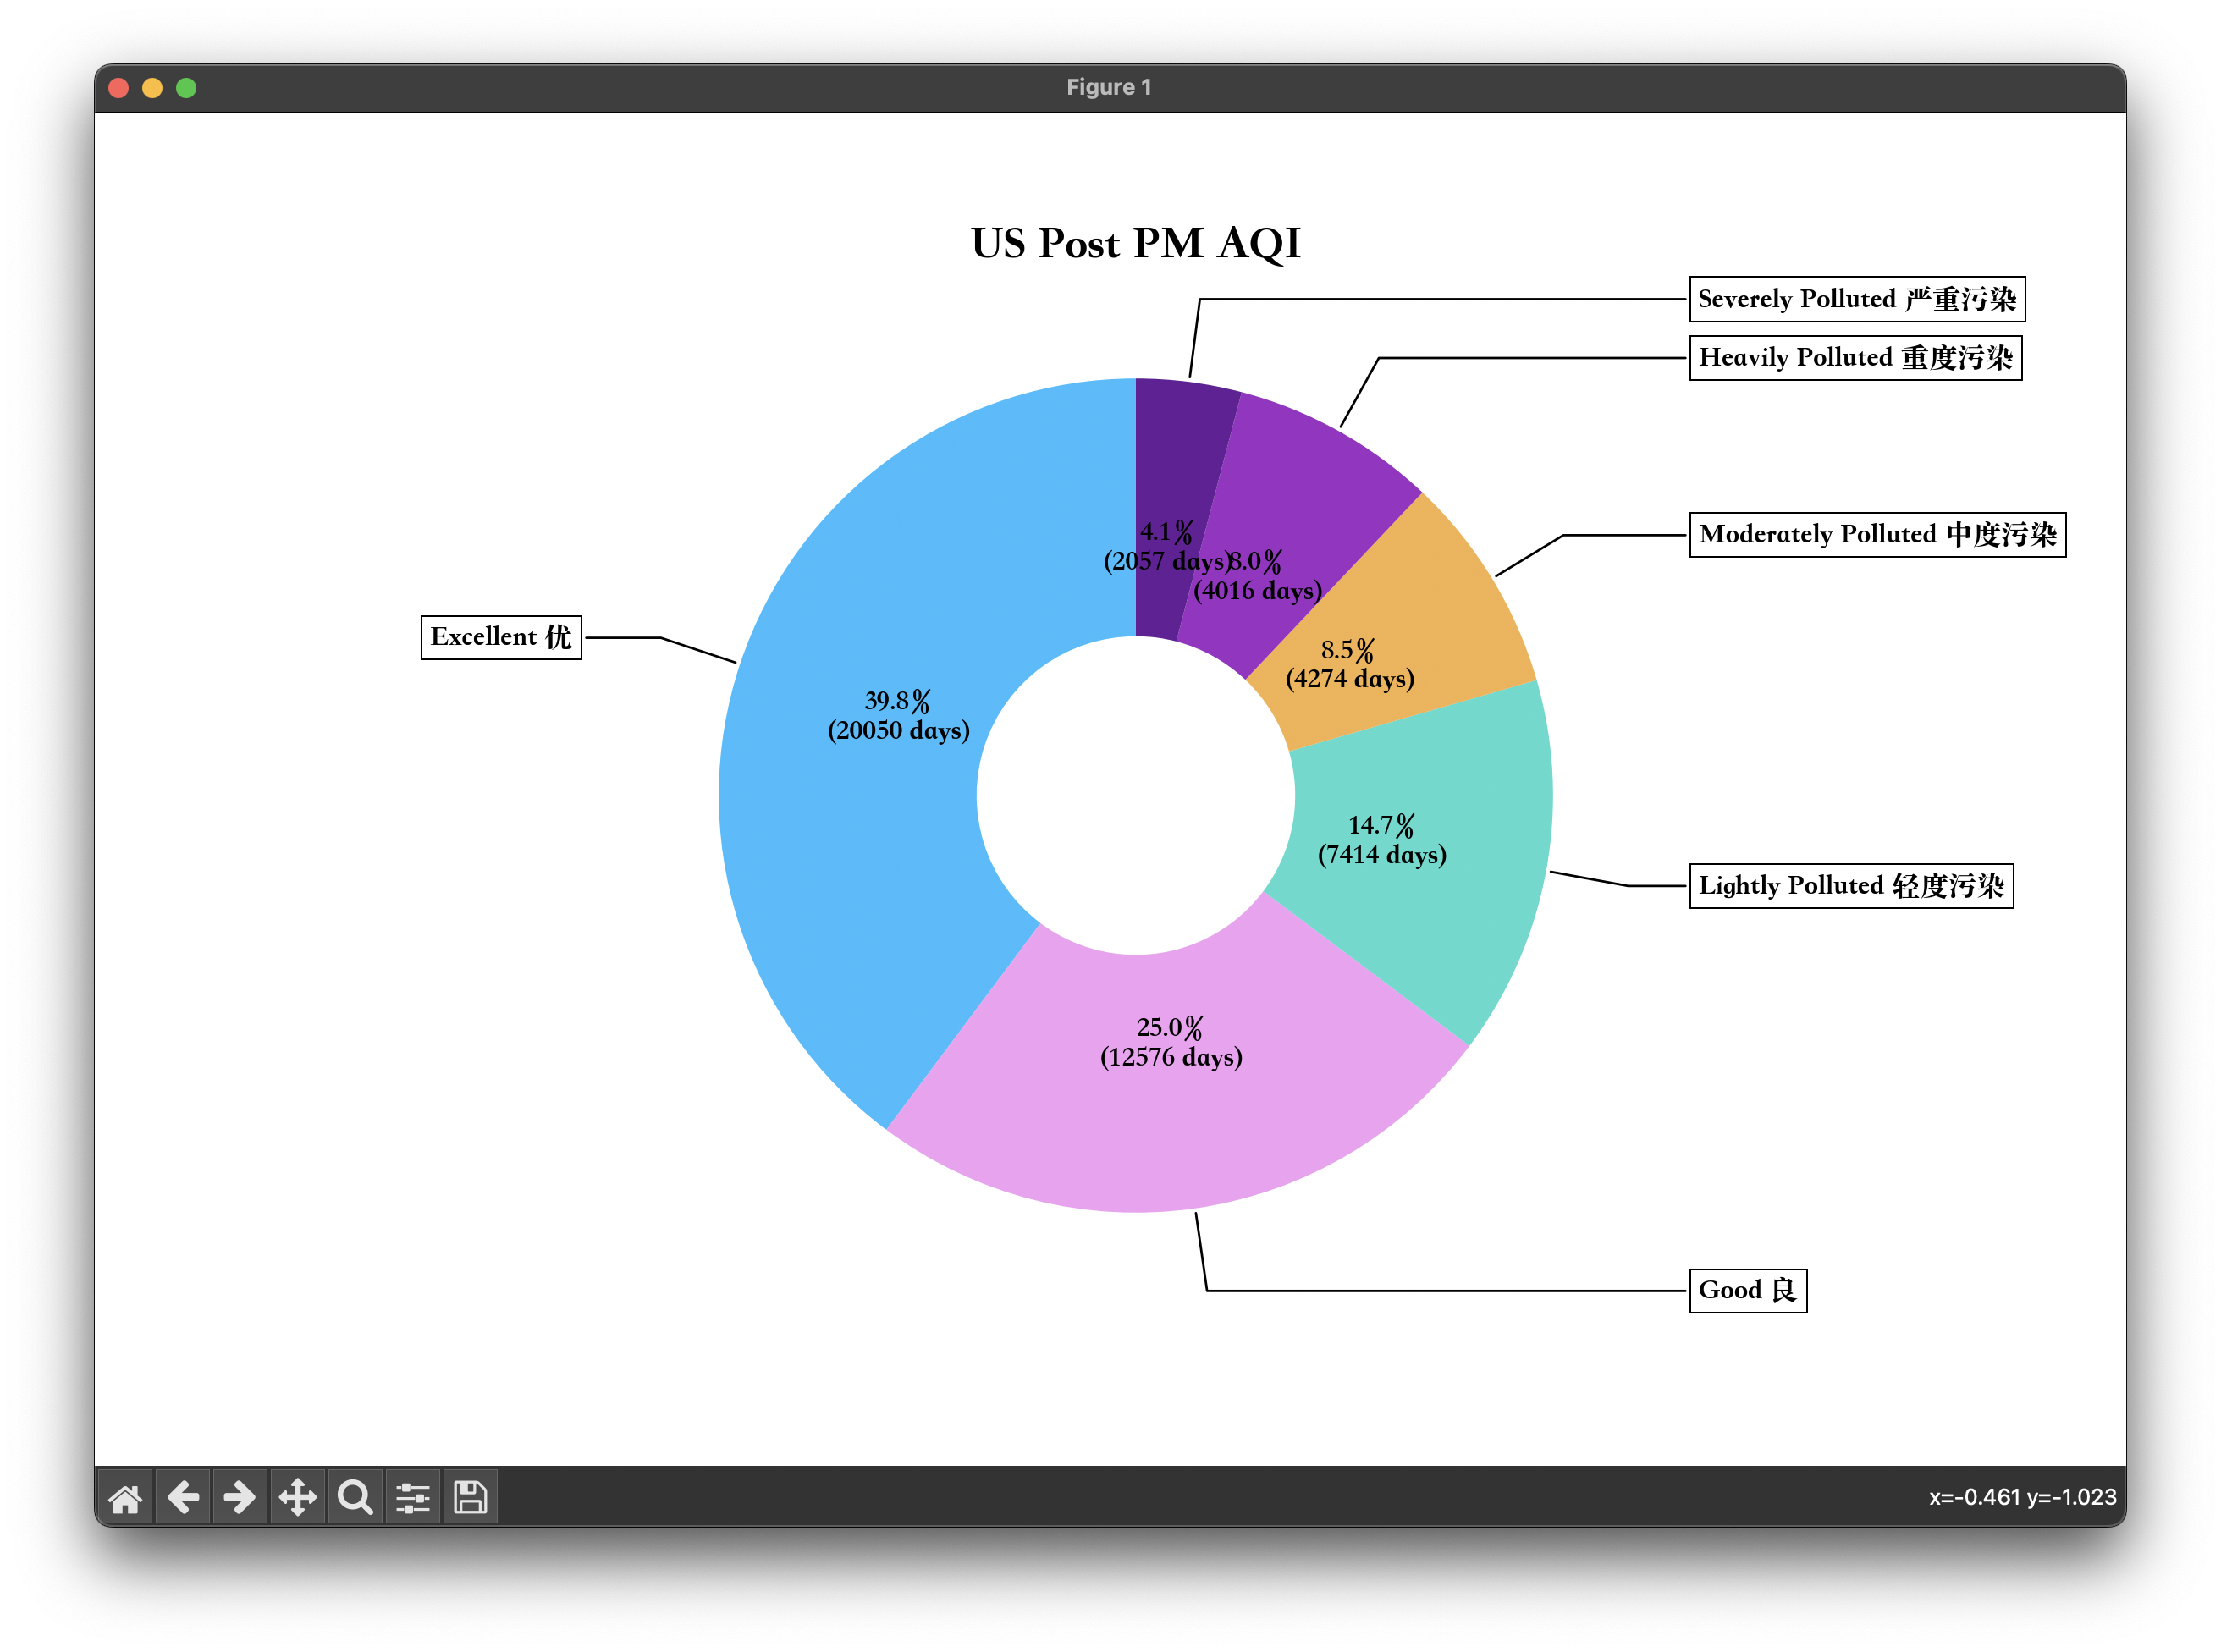
\includegraphics[width=0.8\textwidth]{discretize-aqi-us-post.png}
    \centering
    \caption{PM\_US Post的AQI离散化}
    \label{fig:PMUS Post的AQI离散化}
\end{figure}
